% Generated by render.py; edit preamble.tex and trace.tikz
\documentclass[border=12pt]{standalone}
\def\pgfsysdriver{pgfsys-dvisvgm.def}
\usepackage[dvisvgm]{xcolor}
\usepackage{xeCJK}
\setCJKmainfont{HaranoAjiGothic-Regular.otf}[BoldFont=HaranoAjiGothic-Bold.otf]
\setCJKsansfont{HaranoAjiGothic-Regular.otf}[BoldFont=HaranoAjiGothic-Bold.otf]
\usepackage{amsmath,amssymb,tikz,lmodern}
\usetikzlibrary{arrows.meta,positioning,calc,fit,backgrounds}
\renewcommand{\familydefault}{\sfdefault}
\definecolor{ink}{HTML}{25322F}
\definecolor{green}{HTML}{246657}
\definecolor{tint}{HTML}{EEF4F0}
\definecolor{soft}{HTML}{C6D2CC}
\definecolor{muted}{HTML}{52615B}
\newif\ifJapanese
\newcommand{\Tx}[2]{\ifJapanese #1\else #2\fi}
\newcommand{\Eff}{\overline{\operatorname{Eff}}}
\newcommand{\heading}[3]{{\color{green}\bfseries #1\quad\Tx{#2}{#3}}\\[5pt]}
% A white rectangle makes the complete citation label clickable, including spaces.
\newcommand{\refurl}[2]{\special{dvisvgm:raw <a xlink:href="#1" target="_blank" rel="noopener noreferrer">}{\setlength{\fboxsep}{0pt}\colorbox{white}{\color{green}\underline{\strut #2}}}\special{dvisvgm:raw </a>}}
\tikzset{
 card/.style={draw=soft,fill=white,rounded corners=2pt,align=left,text=ink,font=\fontsize{10.5}{14}\selectfont,inner xsep=12pt,inner ysep=10pt,text width=14.4cm},
 half/.style={card,text width=6.45cm,minimum height=2.05cm},
 result/.style={card,draw=green,fill=tint,line width=.9pt},
 reason/.style={align=left,text=muted,font=\fontsize{9}{12}\selectfont,inner sep=0pt,text width=12.6cm},
 branchreason/.style={reason,text width=5.95cm},
 edge/.style={-{Stealth[length=2.4mm]},draw=green,line width=1pt},
 wire/.style={draw=green,line width=1pt},
}
% Keep the arrow in a dedicated left gutter; explanations never cover it.
\def\flow#1#2#3;{
 \coordinate (#2-from) at ($(#1.south)+(-6.9,0)$);
 \coordinate (#2-to) at ($(#2.north)+(-6.9,0)$);
 \draw[edge] (#2-from)--(#2-to);
 \node[reason,anchor=west] (#2-reason) at ($(#2-from)!.5!(#2-to)+(.55,0)$) {#3};
}

% Style adapted from the repository's Schnell diagrams; MIT attribution retained.
\newcommand{\PRef}[1]{\refurl{https://github.com/openai/math/blob/fd4aeeb2ee4fc729c18d98444fed42fd0529eeeb/preprints/The-Generalized-Mukai-Conjecture-September-24-2026/article.pdf}{#1}}
\newcommand{\MMRef}[1]{\refurl{https://arxiv.org/pdf/math/0409569v4\string##page=5}{#1}}
\newcommand{\TZRef}[1]{\refurl{https://arxiv.org/pdf/1209.4342v5\string##page=4}{#1}}
\newcommand{\KMRef}[1]{\refurl{https://www.ihes.fr/~maxim/TEXTS/relation_between_23.pdf\string##page=7}{#1}}
\newcommand{\PARef}[1]{\refurl{https://www.numdam.org/item/SB_1997-1998__40__307_0.pdf\string##page=6}{#1}}
\newcommand{\BCRef}[1]{\refurl{https://druel.perso.math.cnrs.fr/textes/mukai.pdf\string##page=23}{#1}}
\newcommand{\ERRef}[1]{\refurl{https://druel.perso.math.cnrs.fr/textes/mukai_erratum.pdf}{#1}}
\newcommand{\OCRef}[1]{\refurl{https://doi.org/10.4153/CMB-2006-028-3}{#1}}

\Japanesefalse
\begin{document}
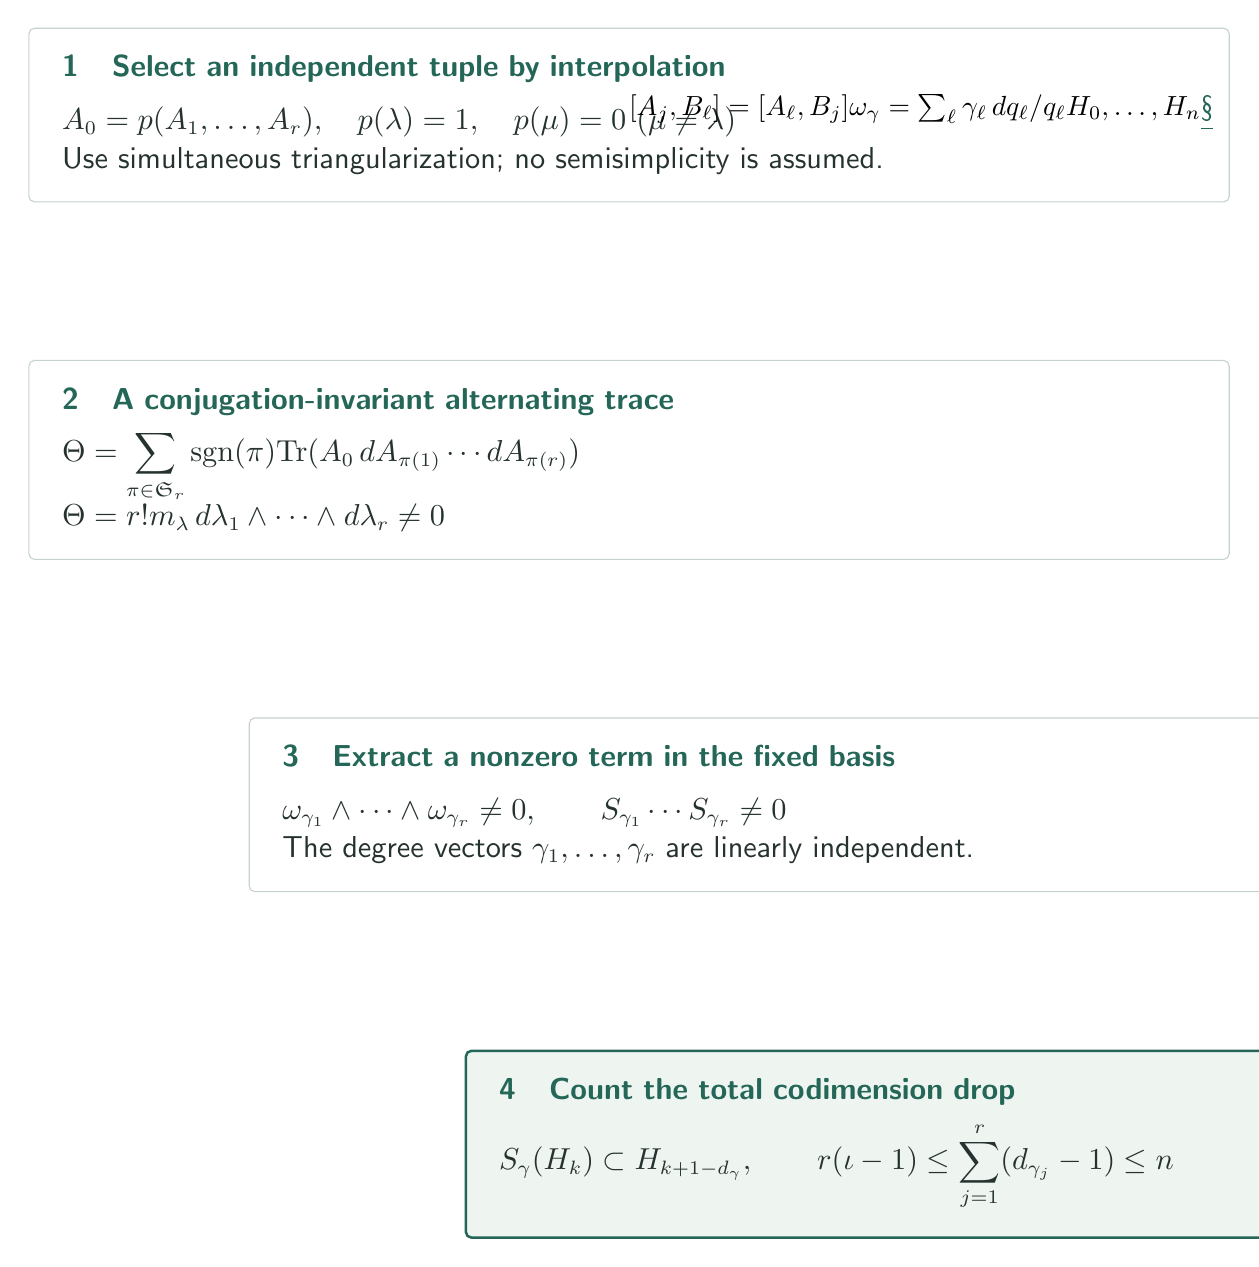
\begin{tikzpicture}

\node[card] (a) {\heading{1}{独立な固有値組を補間で選ぶ}{Select an independent tuple by interpolation}
$A_0=p(A_1,\ldots,A_r),\quad p(\lambda)=1,\quad p(\mu)=0\ (\mu\ne\lambda)$\\
\Tx{同時上三角化を用い、半単純性は仮定しない}{Use simultaneous triangularization; no semisimplicity is assumed.}};
\node[card,below=2cm of a] (b) {\heading{2}{共役に不変な交代トレース}{A conjugation-invariant alternating trace}
$\displaystyle \Theta=\sum_{\pi\in\mathfrak S_r}\mathrm{sgn}(\pi)\mathrm{Tr}(A_0\,dA_{\pi(1)}\cdots dA_{\pi(r)})$\\
$\Theta=r!m_\lambda\,d\lambda_1\wedge\cdots\wedge d\lambda_r\ne0$};
\flow{a}{b}{\Tx{基底の微分が作る交換子項を置換ごとに相殺：}{Pair permutations to cancel the commutators from differentiating the basis:}\\
\PRef{Lemmas 5.1--5.2, pp. 13--15}\quad $[A_j,B_\ell]=[A_\ell,B_j]$};
\node[card,below=2cm of b] (c) {\heading{3}{固定基底で非零項を抽出}{Extract a nonzero term in the fixed basis}
$\omega_{\gamma_1}\wedge\cdots\wedge\omega_{\gamma_r}\ne0,
\qquad S_{\gamma_1}\cdots S_{\gamma_r}\ne0$\\
\Tx{次数ベクトル $\gamma_1,\ldots,\gamma_r$ は線形独立}{The degree vectors $\gamma_1,\ldots,\gamma_r$ are linearly independent.}};
\flow{b}{c}{\Tx{展開して、外積とトレースがともに非零の項を取る：}{Expand and choose a term with both wedge and trace nonzero:}\\
$\omega_\gamma=\sum_\ell\gamma_\ell\,dq_\ell/q_\ell$,\quad \PRef{Prop. 5.3, (15), p. 15}};
\node[result,below=2cm of c] (d) {\heading{4}{余次元の減少量を数える}{Count the total codimension drop}
$S_\gamma(H_k)\subset H_{k+1-d_\gamma},\qquad
\displaystyle r(\iota-1)\le\sum_{j=1}^r(d_{\gamma_j}-1)\le n$};
\flow{c}{d}{\Tx{作用素積が非零なら、総減少量は $H_0,\ldots,H_n$ の幅以下：}{A nonzero product cannot lower degree beyond the range $H_0,\ldots,H_n$:}\\
\PRef{\S2, pp. 3--4; Prop. 5.3, p. 15}};

\end{tikzpicture}
\end{document}
